% Informe del Taller 1 · NovaRetail 360.  Compilar desde esta carpeta:  make informe   (ver ../Makefile)
\documentclass[11pt,letterpaper]{article}
\usepackage{ud-informe}
\usepackage{amsmath}
\setlength{\headheight}{22pt}
\lstdefinelanguage{SQLUD}{morekeywords={SELECT,FROM,JOIN,LEFT,INNER,ON,WHERE,GROUP,BY,ORDER,HAVING,LIMIT,WITH,AS,CASE,WHEN,THEN,ELSE,END,
  SUM,COUNT,ROUND,COALESCE,NULLIF,DISTINCT,OVER,IS,NULL,OR,AND,DESC,CREATE,TABLE,PRIMARY,KEY,REFERENCES,CHECK,NOT,INTEGER,TEXT,REAL},
  sensitive=false, morecomment=[l]{--}, morestring=[b]'}

\renewcommand{\UDtitulo}{NovaRetail 360}
\renewcommand{\UDsubtitulo}{Perfilamiento y limpieza con Power Query, modelo relacional y SQL para inteligencia de negocios}
\renewcommand{\UDtipo}{Taller 1 -- Laboratorio de guía}
\renewcommand{\UDasignatura}{Inteligencia de Negocios}
\renewcommand{\UDdocente}{Nancy Yaneth Gelvez Garcia}
\renewcommand{\UDestudiantes}{Juan Felipe Rodríguez Galindo -- 20261595004}
\renewcommand{\UDencabezado}{Taller 1 -- NovaRetail 360}

\newcommand{\cop}[1]{\$\,#1}
\newcommand{\rojo}[1]{{\color{udrojoosc}\bfseries #1}}

\begin{document}
\UDportada
\tableofcontents
\newpage

%=============================================================================
\section{Resumen ejecutivo}

NovaRetail 360 es un caso ficticio de comercio minorista con seis meses de ventas (enero a junio de 2026).
La gerencia necesita ventas netas, devoluciones, mezcla de canales, cumplimiento de metas y comportamiento
regional, pero los archivos recibidos traen errores de calidad. Este informe documenta cómo se depuraron los
datos, cómo se modeló la información y qué dicen los números una vez depurados.

\begin{itemize}
  \item \textbf{Calidad.} De 1\,201 filas de ventas se aceptaron 1\,193. Se corrigieron 5 por reglas
        deterministas o con evidencia, se apartaron 8 a una tabla de auditoría (ninguna se borró) y se
        registraron 13 incidencias con regla, evidencia, impacto y decisión.
  \item \textbf{Ventas netas.} \cop{699,4} millones, \cop{736,9} millones brutos; el descuento promedio
        efectivo es 5,09\,\%.
  \item \textbf{Metas.} \rojo{Ninguna} de las 30 combinaciones mes--región alcanza su meta; el cumplimiento
        global es 40,8\,\%, y varía muy poco entre regiones (38,7\,\% a 41,8\,\%).
  \item \textbf{Devoluciones.} 4,15\,\% de las unidades (4,28\,\% del valor); Tecnología concentra el
        problema con 6,10\,\%.
  \item \textbf{Canales.} Web, Marketplace y Tienda pesan prácticamente lo mismo (33,5\,\%, 33,5\,\% y 33,0\,\%).
\end{itemize}

\textbf{Recomendación.} Antes de juzgar a las regiones, validar con el negocio cómo se definió la meta: un
cumplimiento uniforme cercano a 40\,\% en todas partes apunta a un problema de escala o de definición de la
meta más que a un problema comercial regional. En paralelo, revisar la calidad y el empaque de la categoría
Tecnología. Las limitaciones (datos sintéticos, seis meses, sin costos) se detallan en la
sección~\ref{sec:indicadores}.

\paragraph{Qué se entrega y qué no.} Se entrega el pipeline reproducible (Python y SQLite), las consultas M de
Power Query equivalentes, la base \texttt{novaretail.db}, la bitácora, el diagrama entidad--relación y las
consultas SQL, y el archivo \texttt{NovaRetail360.pbix} con las 8 consultas, 7 relaciones, 13 medidas y un informe
de tres páginas (resumen ejecutivo, cumplimiento de metas y calidad de datos). Al ejecutar las consultas M en
Power BI Desktop apareció una incidencia que la primera versión del pipeline no detectaba (la fecha inexistente
\texttt{2026-02-30} de V00312); se corrigió el pipeline y todas las cifras de este informe ya la incluyen.

%=============================================================================
\section{Datos y método}

\begin{table}[H]
\centering
\caption{Archivos recibidos.}
\begin{tabularx}{\linewidth}{l r L}
\toprule
Archivo & Filas & Contenido \\
\midrule
\texttt{ventas\_sucias.csv} & 1\,201 & Transacciones: fecha, cliente, producto, canal, cantidad, precio, descuento \\
\texttt{clientes.csv} & 120 & Maestro con región (5) y segmento (Persona/Corporativo) \\
\texttt{productos.csv} & 40 & Catálogo con categoría (4) y precio de lista \\
\texttt{devoluciones.csv} & 70 & Unidades devueltas por venta, con motivo (Defecto/Cambio) \\
\texttt{metas.csv} & 30 & Meta de ventas por mes y región (6 meses $\times$ 5 regiones) \\
\bottomrule
\end{tabularx}
\end{table}

El flujo es el mismo en todo el trabajo: se perfilan los datos, se aplican reglas explícitas, se separa lo
rechazado en lugar de borrarlo y se verifica que \emph{aceptadas + rechazadas = crudas}
($1\,193 + 8 = 1\,201$).

\begin{figure}[H]
\centering
\begin{tikzpicture}[node distance=0.55cm]
  \node[caja] (a) {CSV\\crudos};
  \node[caja, right=of a] (b) {Perfilamiento\\y reglas R1--R9};
  \node[hecho, right=of b] (c) {Ventas\\limpias};
  \node[caja, below=0.5cm of c] (d) {Auditoría\\(8 rechazadas)};
  \node[caja, right=of c] (e) {SQLite\\operacional};
  \node[caja, right=of e] (f) {Esquema\\estrella};
  \draw[flecha] (a) -- (b); \draw[flecha] (b) -- (c); \draw[flecha] (b) |- (d);
  \draw[flecha] (c) -- (e); \draw[flecha] (e) -- (f);
\end{tikzpicture}
\caption{Flujo de depuración y carga.}
\end{figure}

%=============================================================================
\section{Parte A -- Perfilamiento y limpieza}

\subsection{Importación y diagnóstico}

Se importaron los cinco archivos y se revisaron tipos, nulos, duplicados, valores inválidos y referencias a
claves inexistentes. Cuatro archivos salieron limpios (clientes, productos, devoluciones y metas: claves únicas,
sin nulos, 30 metas sin huecos y las 70 devoluciones con venta y cantidad devuelta menor o igual a la vendida).
Todas las incidencias están en \texttt{ventas\_sucias.csv}.

\subsection{Bitácora de calidad}

\begin{table}[H]
\centering
\caption{Bitácora de calidad: una fila por incidencia (detalle y evidencia en \texttt{salida/bitacora\_calidad.csv}).}
\footnotesize
\begin{tabularx}{\linewidth}{r l l l L l}
\toprule
\# & Venta & Regla & Valor observado & Decisión & Acción \\
\midrule
1 & V00016 & R2 formato fecha & \texttt{15/02/2026} & Convertir a \texttt{2026-02-15}; día $>$12 solo admite dd/mm & Corregida \\
2 & V00039 & R2 fecha obligatoria & vacío & Rechazar; no se inventa una fecha & Auditoría \\
3 & V00054 & R3 cliente & \texttt{C9999} & Rechazar; clave inexistente en el maestro & Auditoría \\
4 & V00073 & R3 producto & \texttt{P999} & Rechazar; clave inexistente en el catálogo & Auditoría \\
5 & V00093 & R4 cantidad $>0$ & $-2$ & Rechazar; podría ser una devolución mal registrada & Auditoría \\
6 & V00116 & R4 cantidad $>0$ & vacío & Rechazar; no hay fuente para recuperarla & Auditoría \\
7 & V00141 & R6 precio $>0$ & vacío & Imputar \texttt{precio\_lista} (179\,400; importe 358\,800) & Corregida \\
8 & V00167 & R5 descuento & 1,25 & Rechazar; recortar sería arbitrario & Auditoría \\
9 & V00186 & R7 canal & \texttt{'web '} & Normalizar a \texttt{Web} (trim + proper case) & Corregida \\
10 & V00213 & R7 canal & \texttt{WEB} & Normalizar a \texttt{Web} & Corregida \\
11 & V00240 & R1 unicidad & fila repetida & Conservar la primera, auditar la segunda & Auditoría \\
12 & V00410 & R6 precio $>0$ & $-20\,000$ & Imputar \texttt{precio\_lista} (289\,600; importe 579\,200) & Corregida \\
13 & V00312 & R2 fecha válida & \texttt{2026-02-30} & Rechazar; la fecha no existe y no se inventa el día & Auditoría \\
\bottomrule
\end{tabularx}
\end{table}

\subsection{Normalización y tipificación}

\begin{itemize}
  \item \textbf{Canal.} Se recortan espacios y se unifica la capitalización. Sin esto aparecerían cinco canales
        (\texttt{Web}, \texttt{web\textvisiblespace}, \texttt{WEB}, \dots) y se partiría la participación.
  \item \textbf{Fechas.} Se convierten a ISO (\texttt{aaaa-mm-dd}). Una sola fecha viene en \texttt{dd/mm/aaaa}
        y se resuelve sin ambigüedad porque el día (15) es mayor que 12. En Power Query la conversión debe
        indicar la cultura explícitamente (\texttt{es-CO}); si se deja la del equipo, un mismo archivo da
        resultados distintos en máquinas distintas.
  \item \textbf{Cantidades, precios y descuentos.} Enteros positivos para cantidad y precio; descuento dentro
        de la escala comercial observada (0, 0,05, 0,10 y 0,15). Los números del CSV usan punto decimal, así que
        se leen con cultura \texttt{en-US}.
\end{itemize}

\paragraph{Precio faltante: por qué se imputa y la cantidad no.} En 1\,198 de 1\,198 ventas con precio válido y
producto existente, el precio unitario coincide exactamente con el \texttt{precio\_lista} del catálogo. Hay
evidencia suficiente para recuperar un precio faltante o negativo desde el catálogo (reglas R6). No hay nada
equivalente para cantidad o descuento, así que esos registros se rechazan.

\subsection{Auditoría de registros}

Los ocho registros rechazados se conservan en \texttt{auditoria\_\allowbreak rechazados.csv} (y en la tabla
\texttt{auditoria\_\allowbreak rechazados} de la base) con su motivo. Ninguna devolución apunta a una venta rechazada.

\begin{table}[H]
\centering
\caption{Registros rechazados por motivo.}
\begin{tabularx}{0.8\linewidth}{L r}
\toprule
Motivo & Registros \\
\midrule
R4 cantidad inválida (V00093, V00116) & 2 \\
R1 venta repetida (V00240) & 1 \\
R2 fecha vacía (V00039) & 1 \\
R2 fecha inexistente (V00312, \texttt{2026-02-30}) & 1 \\
R3 \texttt{id\_cliente} inexistente (V00054) & 1 \\
R3 \texttt{id\_producto} inexistente (V00073) & 1 \\
R5 descuento fuera de rango (V00167) & 1 \\
\midrule
\textbf{Total} & \textbf{8} \\
\bottomrule
\end{tabularx}
\end{table}

\subsection{Variables calculadas y política de devoluciones}

\begin{align*}
\text{importe\_bruto} &= \text{cantidad} \times \text{precio\_unitario}\\
\text{importe\_neto} &= \text{importe\_bruto} \times (1-\text{descuento})
\end{align*}

\textbf{Política de devoluciones.}
(1) Las devoluciones \emph{no se restan} del importe neto de la venta: \texttt{importe\_neto} sigue siendo lo
facturado. (2) Cada devolución se vincula a su \textbf{venta original} y su valor es
$\text{unidades devueltas}\times\text{precio}\times(1-\text{descuento})$ de esa venta; así no se suman importes dos
veces. (3) La tasa de devolución se mide \textbf{en unidades} (unidades devueltas / unidades vendidas), no en
transacciones, porque una venta de seis unidades con una devuelta no es una transacción perdida. (4) El valor
devuelto se reporta aparte (4,28\,\% de las ventas netas) para quien necesite una cifra neta de devoluciones
(\cop{670,0} millones).

\subsection{Conciliación: el total casi no cambia, la composición sí}

\begin{table}[H]
\centering
\caption{Puente de conciliación entre la lectura ingenua del archivo y el conjunto depurado (pesos).}
\begin{tabularx}{\linewidth}{L r}
\toprule
Concepto & Importe neto \\
\midrule
Suma ingenua del archivo (blancos $=0$, sin validar) & 701\,679\,450 \\
Quitar venta repetida V00240 & $-1\,015\,920$ \\
Quitar cliente inexistente V00054 & $-1\,476\,960$ \\
Quitar producto inexistente V00073 & $-547\,200$ \\
Quitar fecha vacía V00039 & $-168\,030$ \\
Quitar cantidad negativa V00093 (restaba) & $+326\,800$ \\
Quitar descuento 125\,\% V00167 (restaba) & $+225\,000$ \\
Imputar precio faltante V00141 (valía 0) & $+358\,800$ \\
Imputar precio negativo V00410 (restaba) & $+619\,200$ \\
Quitar fecha inexistente V00312 (\texttt{2026-02-30}) & $-625\,480$ \\
\midrule
\textbf{Conjunto depurado} & \textbf{699\,375\,660} \\
\bottomrule
\end{tabularx}
\end{table}

La diferencia total es de solo 0,33\,\%, porque unos errores suman y otros restan. Por eso no sirve validar un
archivo mirando su total: los errores quedan escondidos hasta que se mira la composición por región, canal o mes.

\subsection{Reproducibilidad}

\textbf{Cómo la garantizan los pasos aplicados.} Power Query guarda cada transformación como una línea de código M
dentro de la consulta (\emph{Applied Steps}). Al llegar un archivo nuevo basta actualizar: se repiten todos los pasos,
en el mismo orden, con las mismas reglas. Esa receta se puede leer, versionar y revisar. En este trabajo la misma
lógica está en \texttt{power\_query/*.pq} y en \texttt{pipeline/limpieza.py}, y las dos producen la partición
aceptadas/rechazadas.

\textbf{Riesgos de reemplazar valores sin una regla documentada.}
\begin{itemize}
  \item \emph{Sesgo silencioso}: reemplazar vacíos por 0 baja promedios y ventas; reemplazar 1,25 por 0,15
        inventa un descuento que nadie aprobó.
  \item \emph{Sin trazabilidad}: el valor original se pierde y nadie puede revisar la decisión.
  \item \emph{Fragilidad}: un reemplazo de un valor literal (``C9999'' por ``C0001'') no se aplica a la siguiente
        entrega, que traerá otros valores sucios, y el proceso falla o, peor, pasa en silencio.
  \item \emph{Dependencia del orden}: cambiar tipos antes de normalizar texto puede producir errores que
        luego se ocultan con \emph{Reemplazar errores}.
\end{itemize}
La alternativa que se adoptó: reglas expresadas como condiciones (no como valores), conservación del registro
original y una consulta de auditoría complementaria.

%=============================================================================
\section{Parte B -- Modelo relacional}

\subsection{Diagrama entidad--relación}

\begin{figure}[H]
\centering
\begin{tikzpicture}[
  ent/.style={draw=udsable!70, fill=white, rounded corners=2pt, font=\footnotesize, inner sep=0pt, minimum width=3.6cm},
  tit/.style={fill=udrojo!10, draw=udsable!70, rounded corners=2pt, font=\small\bfseries\cambria, minimum width=3.6cm, minimum height=0.55cm},
  card/.style={font=\scriptsize\bfseries, color=udrojoosc, fill=white, inner sep=1pt}]
  % clientes
  \node[tit] (tc) at (0,0) {clientes};
  \node[ent, below=0pt of tc, align=left, inner sep=3pt] (c) {\textbf{PK} id\_cliente\\nombre\\region\\segmento};
  % productos
  \node[tit] (tp) at (11,0) {productos};
  \node[ent, below=0pt of tp, align=left, inner sep=3pt] (p) {\textbf{PK} id\_producto\\nombre\_producto\\categoria\\precio\_lista};
  % ventas
  \node[tit, fill=udrojo!22] (tv) at (5.5,-3.1) {ventas \textit{(hecho)}};
  \node[ent, below=0pt of tv, align=left, inner sep=3pt] (v) {\textbf{PK} id\_venta\\\textbf{FK} id\_cliente\\\textbf{FK} id\_producto\\fecha, canal, cantidad\\precio\_unitario, descuento};
  % devoluciones
  \node[tit] (td) at (5.5,-7.4) {devoluciones};
  \node[ent, below=0pt of td, align=left, inner sep=3pt] (d) {\textbf{PK} id\_devolucion\\\textbf{FK} id\_venta\\cantidad\_devuelta\\motivo};
  % metas
  \node[tit] (tm) at (0,-5.6) {metas};
  \node[ent, below=0pt of tm, align=left, inner sep=3pt] (m) {\textbf{PK} (periodo, region)\\meta\_ventas};
  \draw[thick, udsable!70] (c.south) -- ++(0,-0.55) -| (tv.west) ;
  \draw[thick, udsable!70] (p.south) -- ++(0,-0.55) -| (tv.east);
  \draw[thick, udsable!70] (v.south) -- (td.north);
  \draw[thick, udsable!70, dashed] (c.south west) ++(0.35,0) -- ++(0,-2.4) -- (tm.north);
  \node[card] at ($(c.south)+(0,-0.55)+(-0.3,0)$) {1};
  \node[card, anchor=east] at ($(tv.west)+(-0.1,0.25)$) {N};
  \node[card] at ($(p.south)+(0.3,-0.55)$) {1};
  \node[card, anchor=west] at ($(tv.east)+(0.1,0.25)$) {N};
  \node[card, anchor=north west] at ($(v.south)+(0.1,-0.02)$) {1};
  \node[card, anchor=south west] at ($(td.north)+(0.1,0.02)$) {0..N};
  \node[font=\scriptsize\itshape, color=udsable, anchor=west, align=left] at (0.4,-4.55) {relación lógica\\por \texttt{region} (sin FK)};
\end{tikzpicture}
\caption{Modelo operacional. Las líneas continuas son claves foráneas; la línea punteada, una relación lógica
por atributo entre \texttt{metas} y la región del cliente.}
\end{figure}

\begin{table}[H]
\centering
\caption{Claves y cardinalidades.}
\begin{tabularx}{\linewidth}{l l L}
\toprule
Relación & Cardinalidad & Lectura \\
\midrule
clientes $\rightarrow$ ventas & 1 : N & Un cliente tiene muchas ventas; toda venta pertenece a un cliente existente \\
productos $\rightarrow$ ventas & 1 : N & Un producto aparece en muchas ventas; toda venta tiene un producto del catálogo \\
ventas $\rightarrow$ devoluciones & 1 : 0..N & Una venta puede tener cero, una o varias devoluciones (en los datos, 70 ventas con una) \\
metas $\leftrightarrow$ clientes & N : M lógica & La meta se define por (mes, región); la región es atributo de cliente, no entidad \\
\bottomrule
\end{tabularx}
\end{table}

La región no tiene tabla propia. Una mejora sencilla del modelo operacional es extraerla a \texttt{regiones} y
que tanto \texttt{clientes} como \texttt{metas} la referencien; así la relación punteada se vuelve una clave foránea
real.

\subsection{Granularidad de \texttt{ventas} y de \texttt{metas}}

\textbf{Ventas:} una fila por transacción (\texttt{id\_venta}), con un producto por transacción. Es el grano más fino
disponible: de él se puede subir a cualquier agregado (día, región, canal, categoría), pero no al revés.

\textbf{Metas:} una fila por mes y región. Si se une \texttt{metas} directamente a cada transacción, el valor de la
meta se repite en cada venta de su mes y región: en promedio 39,8 veces. Al sumar la meta sobre ese resultado, el
total deja de ser \cop{1\,715} millones y pasa a \cop{68\,322} millones, es decir 39,8 veces más (se verificó
en la base). El mismo error afecta a cualquier unión entre tablas de granularidad distinta: se llama
\emph{fan-out}. La regla es agregar las ventas al grano de la meta (mes, región) \emph{antes} de unir.

\subsection{Operacional frente a estrella}

\begin{table}[H]
\centering
\caption{Comparación de los dos modelos.}
\begin{tabularx}{\linewidth}{l L L}
\toprule
Aspecto & Operacional normalizado & Esquema estrella \\
\midrule
Objetivo & Capturar transacciones sin redundancia ni anomalías & Responder preguntas analíticas con pocas uniones \\
Estructura & 5 tablas en 3FN, uniones por FK & 3 hechos (ventas, devoluciones, metas) y 4 dimensiones (fecha, cliente, producto, canal) \\
Consultas típicas & Varias uniones; el analista debe conocer el modelo & Hecho + dimensiones; atributos listos para filtrar (región, mes, categoría) \\
Escritura & Eficiente y consistente & Se carga por lotes; admite redundancia en dimensiones \\
Metas & Se unen con cuidado (distinto grano) & Hecho propio al grano mes--región; se compara por dimensiones conformadas (región, mes) \\
Riesgo & Fan-out por olvidar el grano & Dimensiones mal conformadas \\
\bottomrule
\end{tabularx}
\end{table}

El esquema estrella está implementado en la base (\texttt{sql/10\_estrella.sql}). Se verificó que
\texttt{fact\_ventas} suma exactamente lo mismo que \texttt{ventas} (diferencia 0).

%=============================================================================
\section{Parte C -- Consultas SQL}

Las consultas completas y comentadas están en el anexo y en \texttt{sql/20\_consultas.sql}. Los resultados vienen
de la base SQLite construida por el equipo con los datos depurados.

\subsection{Consultas de la guía}

\textbf{Q1. Ventas netas por región y mes.} Se une \texttt{ventas} con \texttt{clientes} para obtener la región.

\begin{table}[H]
\centering
\caption{Q1: ventas netas por región y mes (millones de pesos).}
\small
\begin{tabularx}{\linewidth}{L r r r r r r r}
\toprule
Región & Ene & Feb & Mar & Abr & May & Jun & Total \\
\midrule
Bogotá & 14,2 & 23,0 & 29,4 & 26,3 & 20,7 & 17,6 & 131,2 \\
Medellín & 20,9 & 16,6 & 24,0 & 31,5 & 16,4 & 28,2 & 137,6 \\
Cali & 27,3 & 23,5 & 30,6 & 21,8 & 20,5 & 24,2 & 147,9 \\
Barranquilla & 22,1 & 23,7 & 19,7 & 22,4 & 27,9 & 24,0 & 139,8 \\
Bucaramanga & 29,1 & 22,8 & 22,2 & 23,6 & 18,1 & 27,1 & 142,8 \\
\midrule
\textbf{Total} & 113,6 & 109,6 & 125,9 & 125,5 & 103,6 & 121,2 & \textbf{699,4} \\
\bottomrule
\end{tabularx}

\end{table}

Acumulado por región frente a la meta (insumo del indicador I1):

\begin{table}[H]
\centering
\caption{Ventas netas por región, enero--junio 2026 (millones de pesos).}
\begin{tabularx}{\linewidth}{L r r r}
\toprule
Región & Ventas netas & Meta & Cumplimiento \\
\midrule
Bucaramanga & 142,8 & 342,0 & 41,8\,\% \\
Cali & 147,9 & 355,0 & 41,7\,\% \\
Bogotá & 131,2 & 317,0 & 41,4\,\% \\
Medellín & 137,6 & 340,0 & 40,5\,\% \\
Barranquilla & 139,8 & 361,0 & 38,7\,\% \\
\midrule
\textbf{Total} & \textbf{699,4} & \textbf{1\,715,0} & \textbf{40,8\,\%} \\
\bottomrule
\end{tabularx}
\end{table}

\textbf{Q2. Cinco productos con mayores ingresos.} Se agrupa por \texttt{id\_producto} (no por nombre).

\begin{table}[H]
\centering
\caption{Top 5 de productos por ingreso neto.}
\begin{tabularx}{0.85\linewidth}{l l l r r}
\toprule
Producto & Nombre & Categoría & Unidades & Ingreso (millones) \\
\midrule
P037 & Producto 037 & Hogar & 160 & 44,8 \\
P035 & Producto 035 & Accesorios & 136 & 36,6 \\
P039 & Producto 039 & Accesorios & 110 & 32,8 \\
P040 & Producto 040 & Tecnología & 109 & 32,8 \\
P038 & Producto 038 & Oficina & 113 & 32,3 \\
\bottomrule
\end{tabularx}
\end{table}

\textbf{Q3. Participación por canal.}

\begin{figure}[H]
\centering
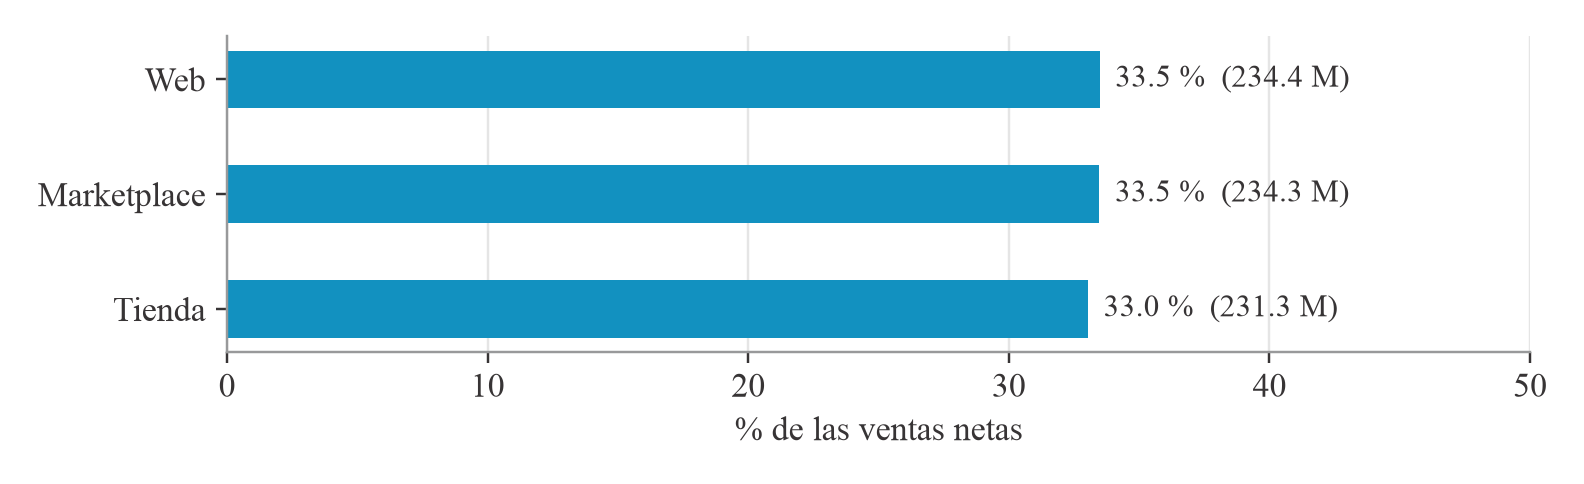
\includegraphics[width=0.82\linewidth]{../salida/figuras/canal.png}
\caption{Participación por canal en las ventas netas.}
\end{figure}

\textbf{Q4. Tasa de devoluciones por unidades.} Se calcula con dos agregaciones independientes que luego se dividen:
174 unidades devueltas sobre 4\,192 vendidas, \textbf{4,15\,\%}. Si se uniera \texttt{devoluciones} a \texttt{ventas} y se
sumara \texttt{cantidad}, una venta con varias devoluciones repetiría sus unidades vendidas. En estos datos cada venta
tiene como máximo una devolución, así que el riesgo no se materializa, pero la consulta se escribió para no depender de eso.

\begin{figure}[H]
\centering
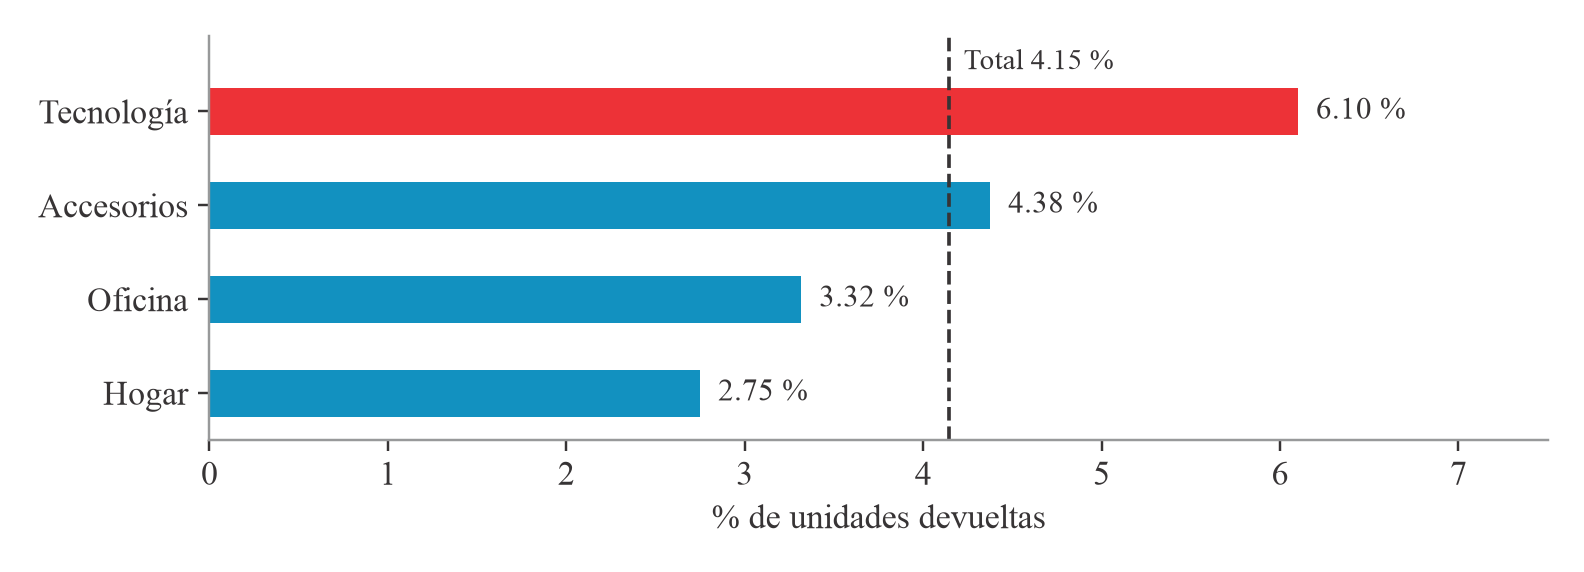
\includegraphics[width=0.82\linewidth]{../salida/figuras/devolucion_categoria.png}
\caption{Tasa de devolución en unidades por categoría.}
\end{figure}

\textbf{Q5. Cumplimiento de metas por mes y región.} Las ventas se agregan a (mes, región) antes de unir con
\texttt{metas} mediante \texttt{LEFT JOIN} desde \texttt{metas}, así una combinación sin ventas aparece con 0\,\% en
vez de desaparecer.

\begin{figure}[H]
\centering
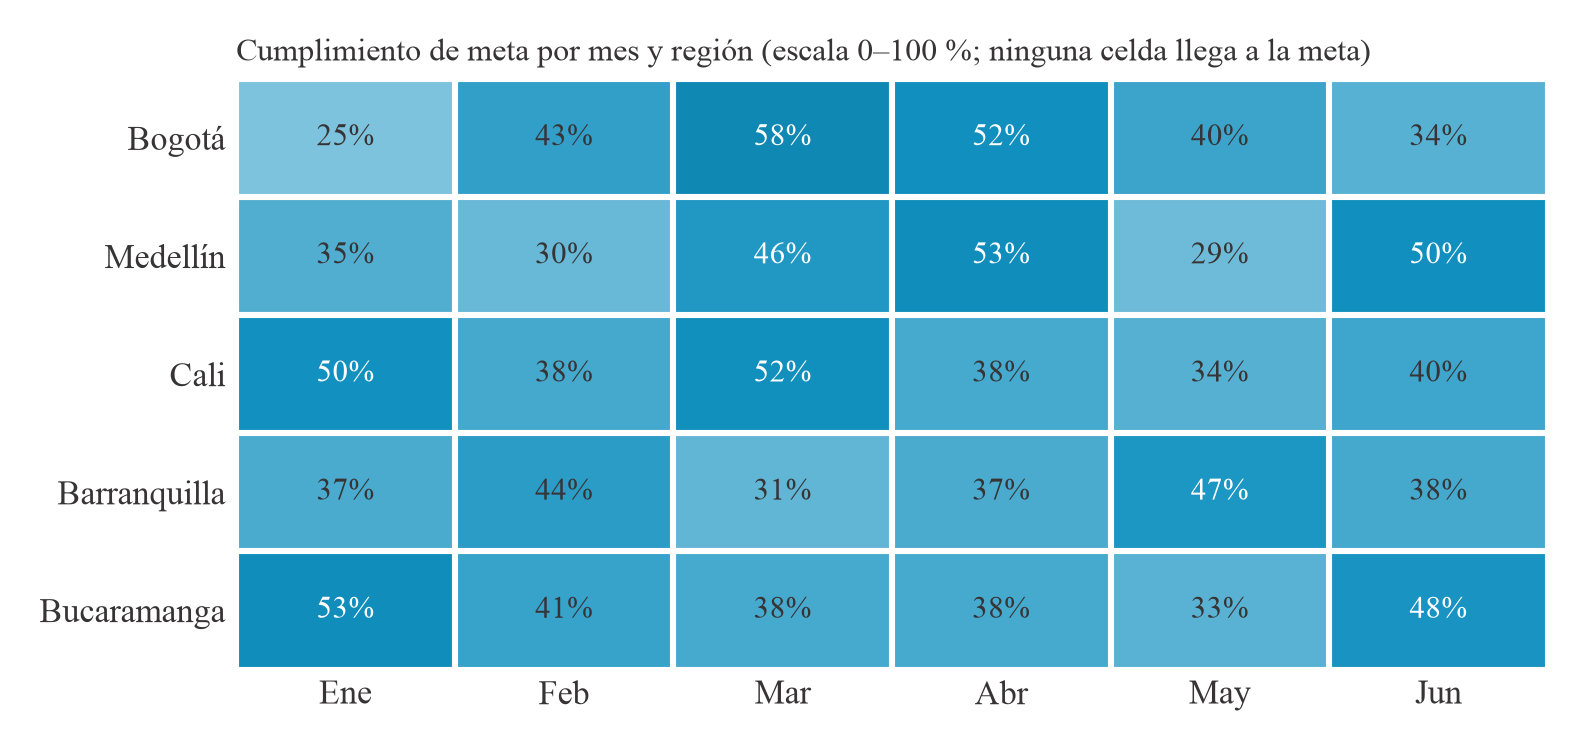
\includegraphics[width=0.92\linewidth]{../salida/figuras/cumplimiento_heatmap.png}
\caption{Cumplimiento de meta. El rango observado es 24,9\,\% (Bogotá, enero) a 57,6\,\% (Bogotá, marzo).}
\end{figure}

\begin{figure}[H]
\centering
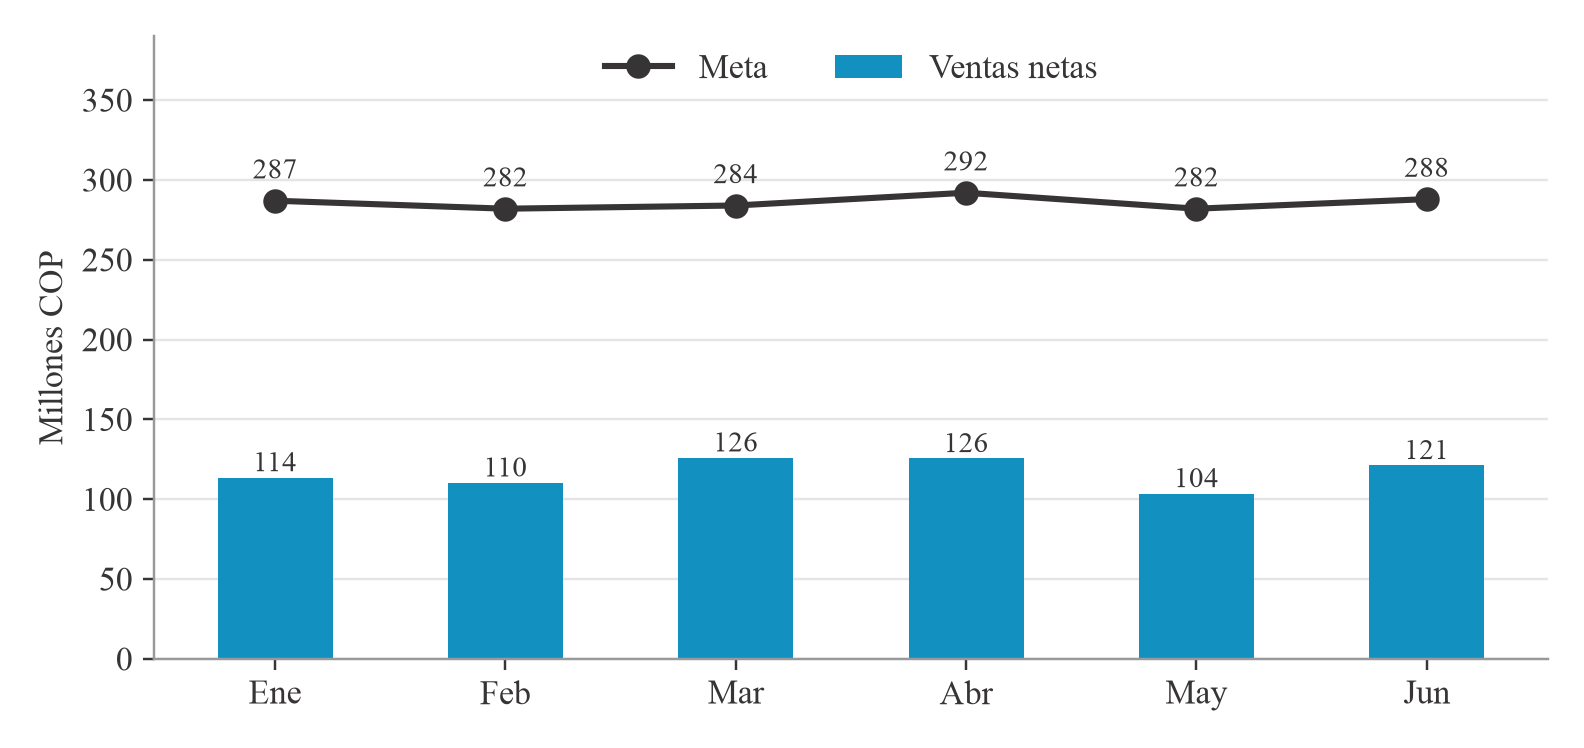
\includegraphics[width=0.82\linewidth]{../salida/figuras/ventas_vs_meta.png}
\caption{Ventas netas frente a meta por mes, todas las regiones (millones de pesos).}
\end{figure}

\subsection{LEFT JOIN, INNER JOIN y calidad de datos}

Sobre los datos \emph{crudos}, un \texttt{LEFT JOIN} desde \texttt{ventas\_crudas} hacia \texttt{clientes} y \texttt{productos},
filtrando donde la clave del lado derecho es nula, devuelve exactamente las dos ventas huérfanas (V00054 con cliente
\texttt{C9999} y V00073 con producto \texttt{P999}). El mismo cruce con \texttt{INNER JOIN} devuelve 1\,199 filas de 1\,201: las dos
desaparecen sin mensaje de error ni advertencia, y los totales salen ``bien'' porque nadie ve lo que falta. Por eso el
\texttt{LEFT JOIN} con prueba de nulos es la herramienta de auditoría, y el \texttt{INNER JOIN} solo se usa cuando la
integridad ya está garantizada (o cuando descartar es la decisión deliberada).

\subsection{\texttt{WHERE} frente a \texttt{HAVING}; \texttt{COUNT(*)} frente a \texttt{COUNT(DISTINCT)}}

\begin{itemize}
  \item \texttt{WHERE} filtra \emph{filas} antes de agrupar; no puede usar funciones de agregación. \texttt{HAVING} filtra
        \emph{grupos} después de agregar. Ejemplo (\texttt{sql/30\_calidad\_y\_conceptos.sql}): con \texttt{WHERE fecha >= '2026-03-01'}
        se descartan las ventas de enero y febrero antes de sumar; con \texttt{HAVING SUM(importe\_neto) > 95\,000\,000}
        solo sobreviven las regiones cuyo total ya agregado supera ese valor (Medellín y Cali).
  \item \texttt{COUNT(*)} cuenta filas; \texttt{COUNT(DISTINCT id\_venta)} cuenta ventas únicas. Sobre las ventas crudas
        da 1\,201 frente a 1\,200: la diferencia es exactamente el duplicado V00240. Tras unir con una tabla de
        relación 1:N (por ejemplo devoluciones múltiples) \texttt{COUNT(*)} sobrecontaría ventas, mientras que
        \texttt{COUNT(DISTINCT id\_venta)} no.
\end{itemize}

\subsection{Verificación cruzada}

El archivo \texttt{consultas\_referencia.sql} que acompaña la guía se ejecutó sobre la base depurada y arroja los
mismos números que las consultas propias en ingreso por región y mes y en cumplimiento de metas.

%=============================================================================
\section{Parte D -- Indicadores y recomendación ejecutiva}
\label{sec:indicadores}

\subsection{Tres indicadores}

\begin{table}[H]
\centering
\caption{Indicadores empresariales.}
\begin{tabularx}{\linewidth}{>{\raggedright\arraybackslash}p{4.3cm} >{\raggedright\arraybackslash}p{3.1cm} L}
\toprule
Indicador & Valor & Lectura \\
\midrule
\textbf{I1. Cumplimiento de metas} (ventas netas / meta) & 40,8\,\% \; (0 de 30 cumplen) &
  Uniforme entre regiones (38,7\,\% a 41,8\,\%); no hay una región ``problema''. \\
\textbf{I2. Tasa de devolución en unidades} & 4,15\,\% \; (valor: 4,28\,\%) &
  Tecnología 6,10\,\%, Accesorios 4,39\,\%, Oficina 3,32\,\%, Hogar 2,75\,\%. Por región, de 2,43\,\% (Bucaramanga) a 4,90\,\% (Cali). \\
\textbf{I3. Mezcla de canales} (participación en ventas netas) & 33,5\,\% / 33,5\,\% / 33,0\,\% &
  Sin dependencia de un canal; ningún canal es la palanca obvia de crecimiento. \\
\bottomrule
\end{tabularx}
\end{table}

Otros datos de contexto: ticket promedio de \cop{586\,233} por transacción, 120 de 120 clientes activos, 55\,\% de
las ventas en el segmento Corporativo (que es la mitad de los clientes), y descuentos por \cop{37,5} millones
(5,09\,\% del bruto).

\subsection{Recomendación ejecutiva}

\begin{enumerate}
  \item \textbf{Revisar la definición de las metas antes de reaccionar.} Las ventas llegan al 41\,\% de la meta en todas
        las regiones y casi en todos los meses; una brecha tan pareja es característica de una meta mal escalada
        (por ejemplo, definida sobre otra base o sobre otro periodo), no de un fallo comercial regional. Hasta
        validarlo, no se recomienda tomar decisiones de personal o de incentivos con este indicador.
  \item \textbf{Investigar las devoluciones de Tecnología.} Es la categoría con 6,10\,\% frente a 4,15\,\% global.
        El motivo se reparte entre \emph{Defecto} y \emph{Cambio} (84 y 90 unidades en total), así que conviene
        cruzar la categoría con el motivo y con el proveedor antes de actuar.
  \item \textbf{Mantener los tres canales} y buscar crecimiento por segmento o categoría, ya que el canal no discrimina.
\end{enumerate}

\subsection{Limitaciones}

\begin{itemize}
  \item \textbf{Datos sintéticos} con incidencias intencionales: las cifras ilustran el método, no el desempeño
        de una empresa real.
  \item \textbf{Seis meses} (enero a junio de 2026): no hay estacionalidad ni comparación interanual.
  \item \textbf{Sin costos}: se mide ingreso, no margen; una categoría con muchas devoluciones puede ser
        más o menos rentable que lo que sugieren sus ingresos.
  \item \textbf{Decisiones de limpieza.} Se rechazaron 8 registros (0,67\,\% de las filas) y se imputaron 2 precios.
        En conjunto, las decisiones mueven el total un 0,33\,\%; aun así, las reglas con rechazo deben confirmarse con el
        dueño del dato.
  \item \textbf{Devoluciones sin fecha}: la tasa se asigna al periodo de la venta original y no se puede
        analizar la demora entre venta y devolución.
  \item \textbf{Validación cruzada}: los guiones M se ejecutaron en Power BI Desktop y reproducen las cifras del pipeline en Python
        (1\,193 ventas y \cop{699\,375\,660} netos); esa ejecución fue la que detectó la fecha inexistente de V00312.
  \item \textbf{Recuperación de precio}: la regla R6 supone que las ventas se facturan a precio de lista; se verificó
        en 1\,198 de 1\,198 casos, pero podría dejar de cumplirse con datos reales.
\end{itemize}

%=============================================================================
\section{Reproducir el trabajo}

\begin{lstlisting}[language=bash,numbers=none]
python3 pipeline/limpieza.py                                   # limpia y crea salida/novaretail.db
uv run --no-project --with matplotlib python pipeline/graficos.py   # figuras + resultados.json
sqlite3 -header -column salida/novaretail.db < sql/20_consultas.sql
make informe presentacion                                     # PDF con la plantilla UD (tectonic)
\end{lstlisting}

\begin{table}[H]
\centering
\caption{Estructura de la entrega.}
\begin{tabularx}{\linewidth}{l L}
\toprule
Ruta & Contenido \\
\midrule
\texttt{pipeline/} & Limpieza (\texttt{limpieza.py}) y figuras (\texttt{graficos.py}) \\
\texttt{power\_query/} & Consultas M equivalentes (ejecutadas en Power BI Desktop) \\
\texttt{NovaRetail360.pbix} & Archivo de Power BI: consultas, modelo, medidas DAX e informe de tres páginas \\
\texttt{sql/} & Esquema, estrella, cinco consultas y consultas de calidad \\
\texttt{salida/} & Datos limpios, auditoría, bitácora, base SQLite, figuras, resultados \\
\texttt{informe/}, \texttt{presentacion/} & Fuentes LaTeX y PDF \\
\texttt{portal/} & Sitio web explicativo \\
\bottomrule
\end{tabularx}
\end{table}

%=============================================================================
\appendix
\section{Consultas SQL comentadas}

\lstinputlisting[language=SQLUD, basicstyle=\ttfamily\scriptsize]{../sql/20_consultas.sql}

\end{document}
